\documentclass[aspectratio=169, 11pt]{beamer}
\usetheme{metropolis}

\usepackage{graphicx}
\usepackage{booktabs}
\usepackage{xcolor}
\usepackage{appendixnumberbeamer}

% Custom colors
\definecolor{alertred}{RGB}{204, 36, 29}
\definecolor{okgreen}{RGB}{40, 140, 40}
\definecolor{noteblue}{RGB}{30, 90, 160}

\setbeamercolor{alerted text}{fg=alertred}

\graphicspath{{figs/}}

\title{PA$\to$NY Pipeline Cap:\\Bug or Economics?}
\subtitle{Diagnostic Investigation of the 4~bcf/day Flow Ceiling}
\author{Caleb Sy}
\date{March 2026}
\institute{PhD Research Briefing}

\begin{document}

\maketitle

%% ============================================================
%% PART I: THE OBSERVATION
%% ============================================================

\section{The Observation}

% ---- Slide 2: Setup ----
\begin{frame}{Context: NE Dual Depression Investigation}
  Prior work (dual drop investigation) found:
  \begin{itemize}
    \item \textbf{30+ pipeline segments} at capacity in Part~3 during injection season
    \item PA$\to$NY cited as \alert{``at 100\% utilization on all 372 days''} --- a key congestion bottleneck driving New England price depression
  \end{itemize}

  \vspace{0.5em}
  \textbf{New question}: The hard pipeline capacity is \textbf{5.060~bcf/day}, \\
  but flows appear to cap at \alert{$\sim$4.048~bcf/day}.

  \vspace{0.5em}
  \begin{block}{Is this a bug or correct behavior?}
    \begin{itemize}
      \item \textbf{Bug hypothesis}: data setup drops or miscodes a tariff step, creating a spurious constraint
      \item \textbf{Economic hypothesis}: the next tariff tier is too expensive --- optimizer stops voluntarily
    \end{itemize}
  \end{block}
\end{frame}

% ---- Slide 3: Tariff Structure ----
\begin{frame}{The Stepped Tariff Structure}
  The raw pipeline tariff CSV has 5 steps. \texttt{v14\_data\_setup\_dev.py} drops step~1 and renumbers steps~2--5 to produce 4 model steps:

  \vspace{0.5em}
  \begin{table}
    \centering
    \begin{tabular}{cccc}
      \toprule
      \textbf{Model step} & \textbf{Cumul.\ cap (bcf)} & \textbf{Tariff (raw)} & \textbf{Tariff $\times$ CPI 2.18} \\
      \midrule
      1 & 2.530 & \$0.05/mmbtu & \$0.109/mmbtu \\
      2 & \textbf{4.048} & \$0.10/mmbtu & \$0.218/mmbtu \\
      \rowcolor{gray!15}
      3 & 5.060 & \alert{\$1.50/mmbtu} & \alert{\$3.27/mmbtu} \\
      4 & 7.083 & \$4.00/mmbtu & \$8.72/mmbtu \\
      \bottomrule
    \end{tabular}
  \end{table}

  \vspace{0.5em}
  Step~3 costs \alert{\$3.27/mmbtu} --- a \textbf{15$\times$ jump} from step~2 (\$0.218/mmbtu). \\
  The optimizer only crosses this threshold when $\text{dual}_\text{NY} - \text{dual}_\text{PA} > \$3.27$.
\end{frame}

% ---- Slide 4: MaxPipe Constraint ----
\begin{frame}{The \texttt{MaxPipe} Constraint}
  In \texttt{v14\_gas\_model\_dev.py} (lines~498--504), each step's flow is bounded
  by its \emph{incremental width}:

  \vspace{0.3em}
  \begin{table}
    \centering
    \small
    \begin{tabular}{cll}
      \toprule
      \textbf{Step} & \textbf{Incremental bound} & \textbf{Value (bcf)} \\
      \midrule
      1 & \texttt{step\_flow}$[\ell,1,t] \leq$ \texttt{FTariff\_CAP}$[\ell,1]$ & 2.530 \\
      2 & \texttt{step\_flow}$[\ell,2,t] \leq$ \texttt{FTariff\_CAP}$[\ell,2]$ $-$ \texttt{FTariff\_CAP}$[\ell,1]$ & 1.518 \\
      3 & \texttt{step\_flow}$[\ell,3,t] \leq$ \texttt{FTariff\_CAP}$[\ell,3]$ $-$ \texttt{FTariff\_CAP}$[\ell,2]$ & 1.012 \\
      4 & \texttt{step\_flow}$[\ell,4,t] \leq$ \texttt{FTariff\_CAP}$[\ell,4]$ $-$ \texttt{FTariff\_CAP}$[\ell,3]$ & 2.024 \\
      \bottomrule
    \end{tabular}
  \end{table}

  \vspace{0.3em}
  Maximum achievable flow using steps~1+2 only:
  \[
    2.530 + 1.518 = \mathbf{4.048~\text{bcf/day}}
  \]
  This exactly matches the observed ``cap.'' Step~3 adds the 5.060~bcf tier at \$3.27/mmbtu.
\end{frame}

%% ============================================================
%% PART II: DIAGNOSTIC RESULTS
%% ============================================================

\section{Diagnostic Results}

% ---- Slide 5: Script 01 ----
\begin{frame}{Script~01: Flow Distribution Over 372 Days}
  \begin{figure}
    \centering
    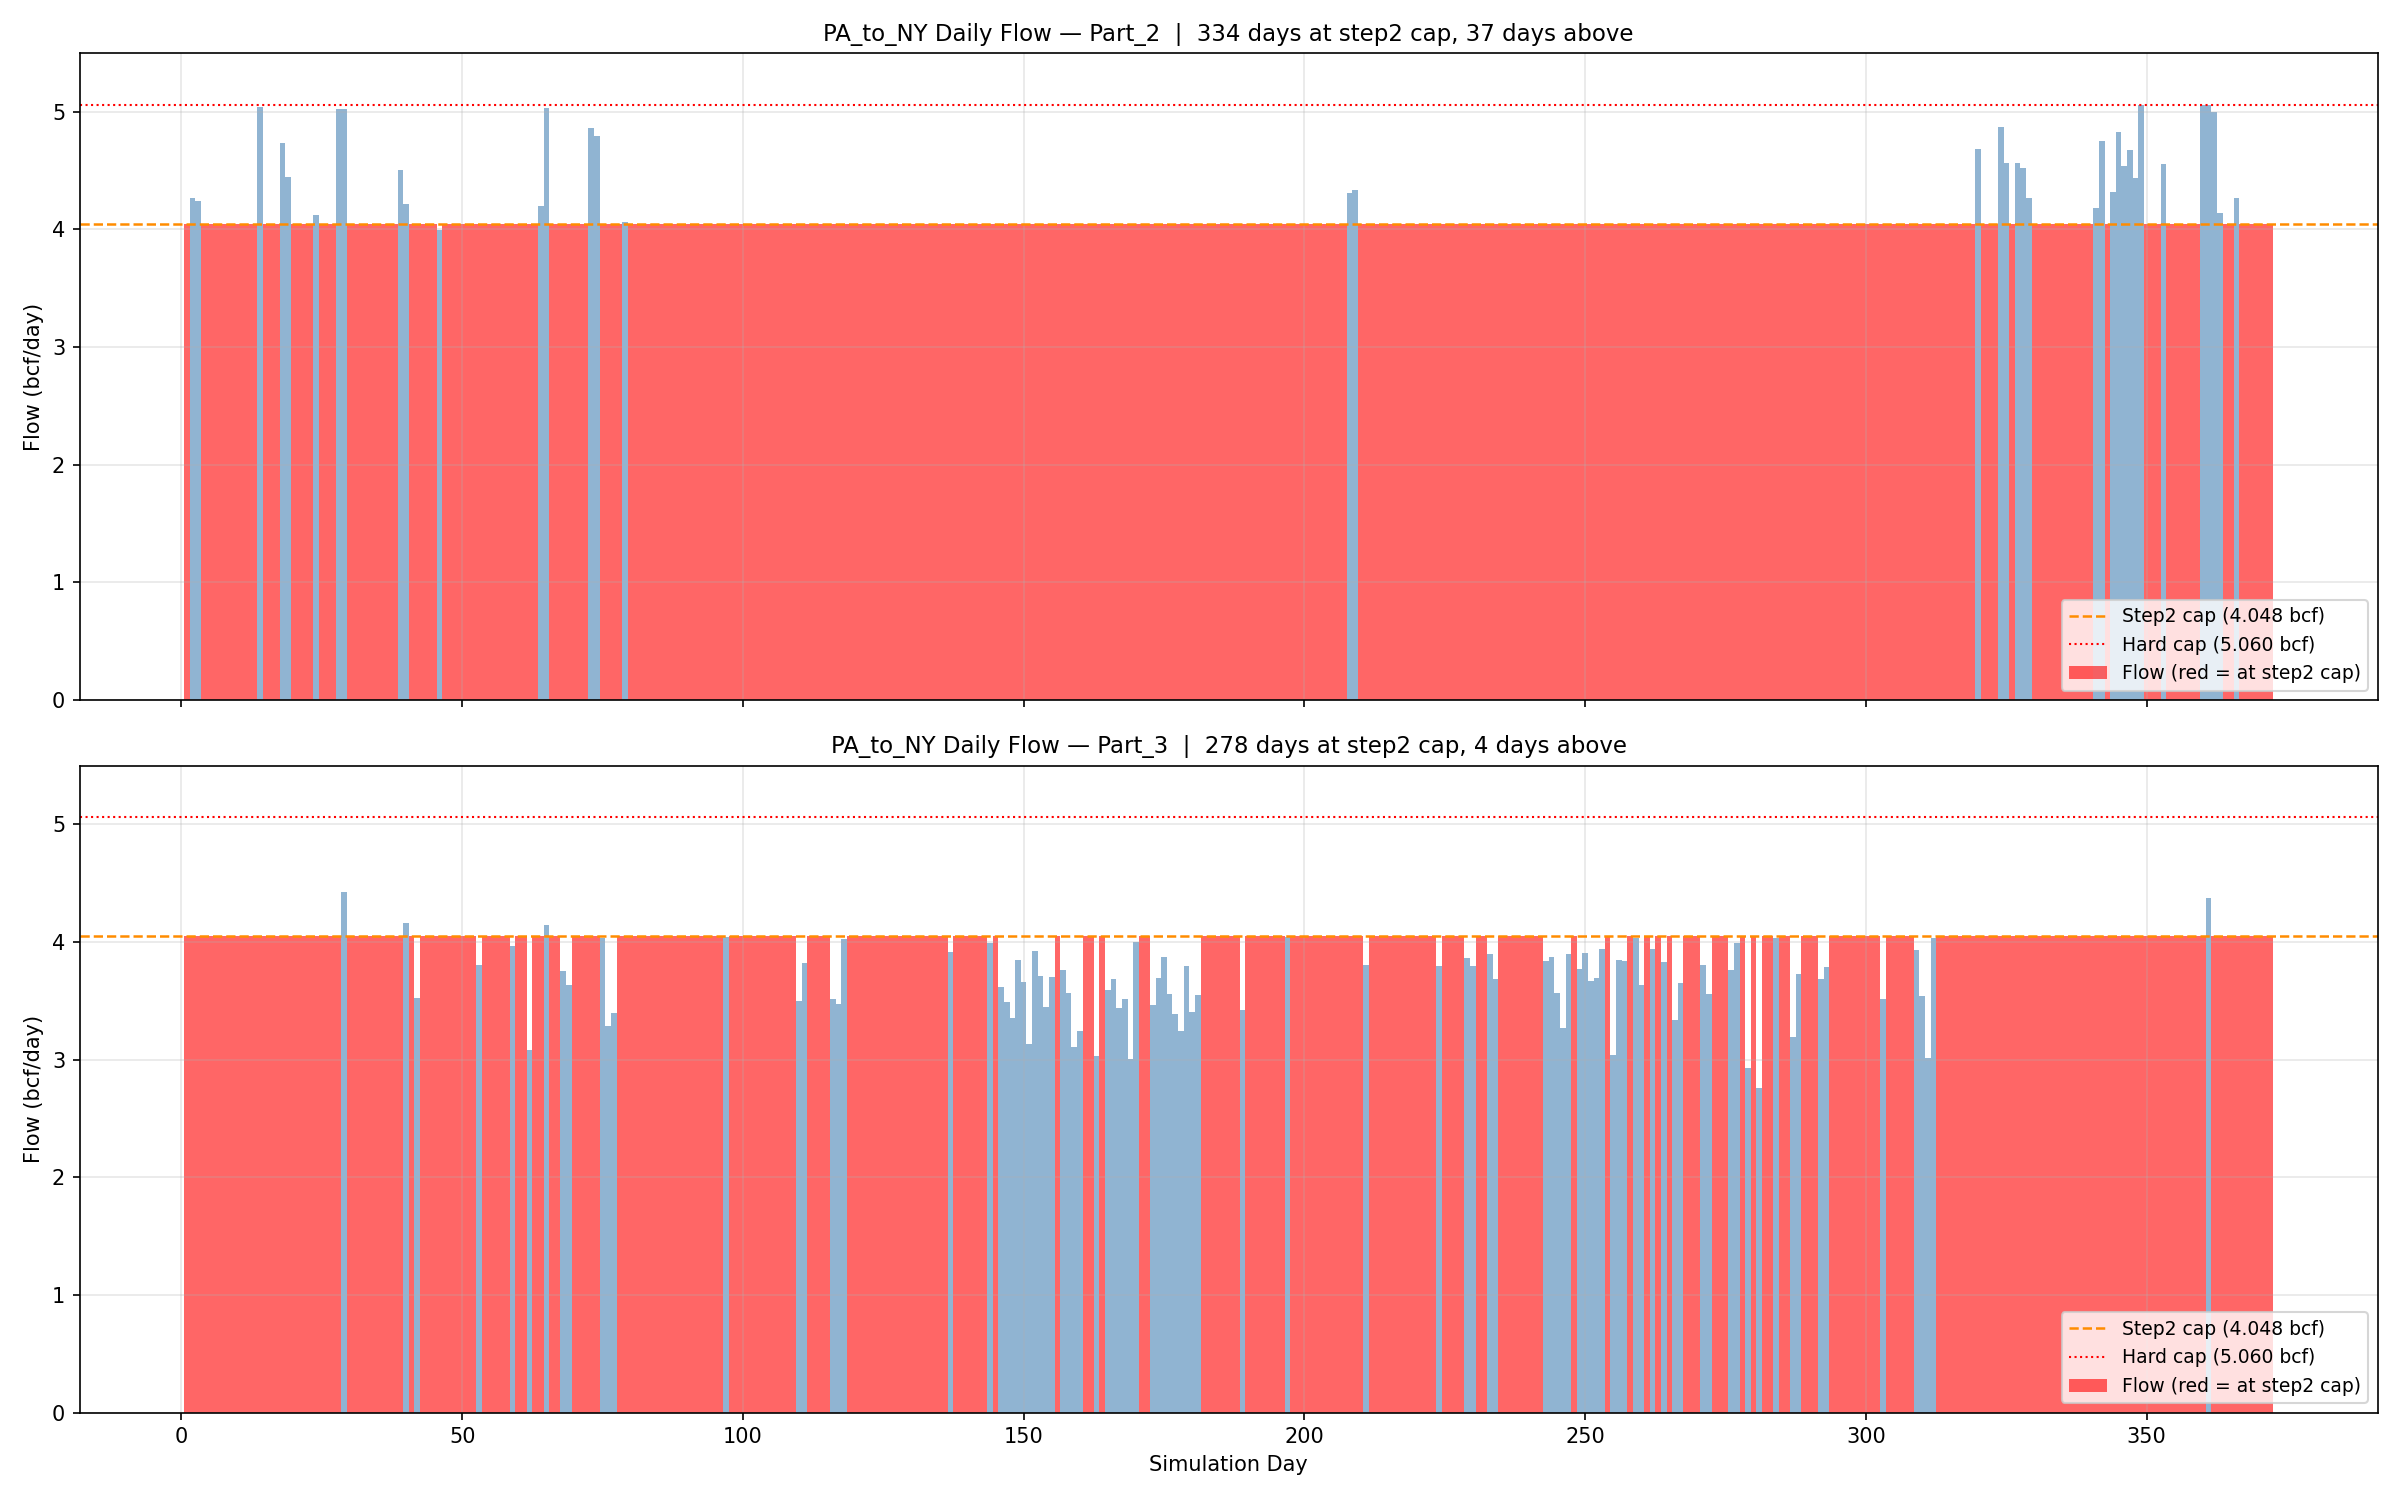
\includegraphics[width=0.90\linewidth]{pipe_01_flow_distribution.png}
  \end{figure}
  \vspace{-0.5em}
  {\small \textbf{Red bars}: days at step~2 cap (4.048~bcf). Reference lines: orange dashed = step~2 cap, red dotted = hard cap (5.060~bcf).
  Part~2 has \textbf{37 days} above step~2 cap --- step~3 capacity \emph{is} being used.}
\end{frame}

% ---- Slide 6: Flow stats table ----
\begin{frame}{Script~01: What the Flows Actually Show}
  \begin{table}
    \centering
    \begin{tabular}{lcc}
      \toprule
      \textbf{Condition} & \textbf{Part~2} & \textbf{Part~3} \\
      \midrule
      At step~2 cap ($\approx$4.048~bcf) & 334 days (89.8\%) & 278 days (74.7\%) \\
      \textbf{Above step~2 cap (step~3 in use)} & \textcolor{okgreen}{\textbf{37 days (9.9\%)}} & \textcolor{okgreen}{\textbf{4 days (1.1\%)}} \\
      Below step~2 cap (demand-limited)  & 1 day (0.3\%)   & 90 days (24.2\%) \\
      At hard cap (5.060~bcf)            & 3 days (0.8\%)  & 0 days \\
      \bottomrule
    \end{tabular}
  \end{table}

  \vspace{0.5em}
  \textbf{Key revision}: The initial observation was slightly off.
  \begin{itemize}
    \item Step~3 \emph{is} used on high-demand days --- the optimizer pays \$3.27/mmbtu when it has to
    \item Most days (89.8\% Part~2) stop at 4.048~bcf not because of a hard constraint, \\
      but because the NY--PA price spread doesn't justify crossing the cost cliff
  \end{itemize}
\end{frame}

% ---- Slide 7: Script 02 ----
\begin{frame}{Script~02: NY--PA Dual Gap vs.\ Tariff Threshold}
  \begin{figure}
    \centering
    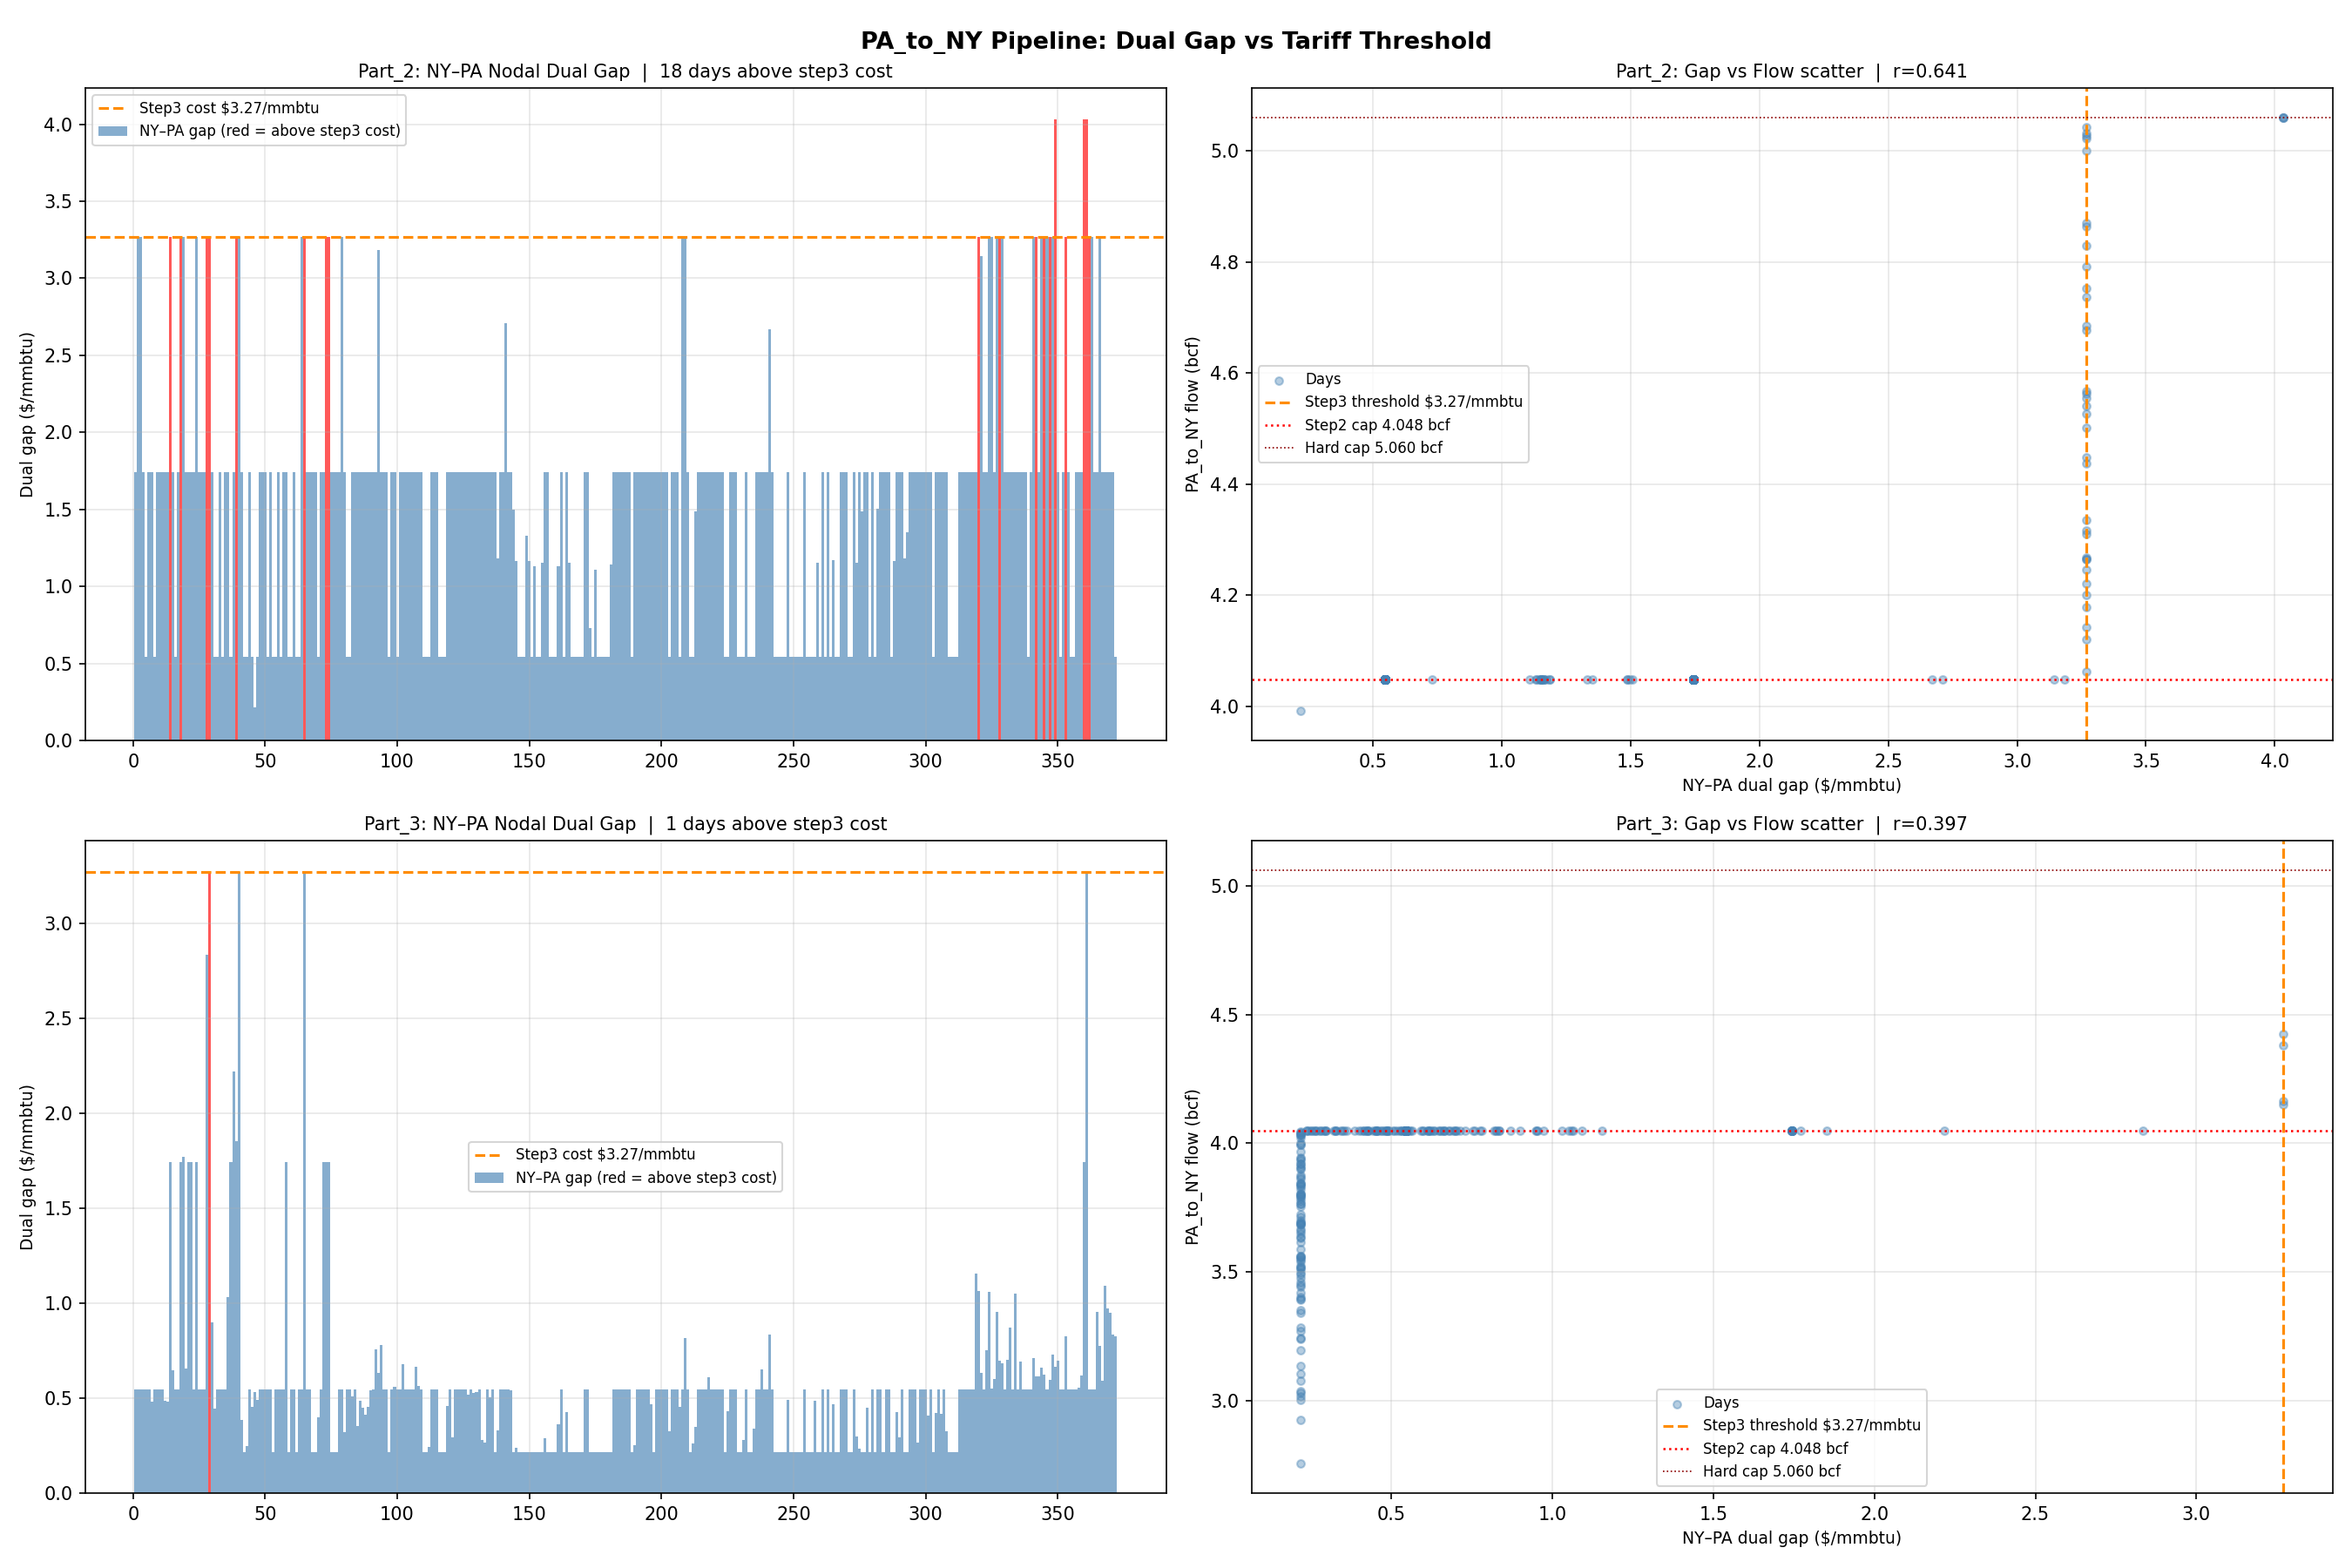
\includegraphics[width=0.90\linewidth]{pipe_02_dual_gap_vs_tariff.png}
  \end{figure}
  \vspace{-0.5em}
  {\small \textbf{Left}: daily NY--PA dual gap (red bars = gap exceeds \$3.27 threshold). \textbf{Right}: scatter of gap vs.\ flow --- all days above the threshold have correspondingly high flows. \alert{Zero conflict days.}}
\end{frame}

% ---- Slide 8: Bug check ----
\begin{frame}{Script~02: The Key Bug Test}
  \textbf{Definition}: A \emph{conflict day} is any day where:
  \[
    \underbrace{\text{dual}_\text{NY} - \text{dual}_\text{PA}}_{\text{willingness to pay}} > \underbrace{\$3.27/\text{mmbtu}}_{\text{step~3 cost}}
    \quad \text{but} \quad
    \underbrace{\text{flow} \leq 4.048~\text{bcf}}_{\text{step~3 not used}}
  \]
  A conflict day would indicate a binding constraint preventing use of economically justified capacity --- i.e., a bug.

  \vspace{0.5em}
  \begin{table}
    \centering
    \begin{tabular}{lcc}
      \toprule
      & \textbf{Part~2} & \textbf{Part~3} \\
      \midrule
      Days with gap $>$ \$3.27/mmbtu    & 18 (4.8\%)  & 1 (0.3\%) \\
      \textbf{Conflict days (BUG indicator)}  & \textcolor{okgreen}{\textbf{0}}     & \textcolor{okgreen}{\textbf{0}} \\
      \bottomrule
    \end{tabular}
  \end{table}

  \vspace{0.5em}
  \begin{block}{Verdict}
    \textbf{No bug.} On every day where the spread exceeds \$3.27/mmbtu, the optimizer correctly uses step~3 capacity. The 4~bcf ``cap'' is entirely structural/economic.
  \end{block}
\end{frame}

% ---- Slide 9: Script 03 ----
\begin{frame}{Script~03: Data File Verification}
  Parsed the Pyomo \texttt{.dat} file (\texttt{model\_DATAFILE\_qps\_0.0\_ftariff\_0.0\_prod\_0.98.dat}) and confirmed PA$\to$NY entries:

  \vspace{0.3em}
  \begin{table}
    \centering
    \small
    \begin{tabular}{ccccc}
      \toprule
      \textbf{Step} & \textbf{.dat cap (bcf)} & \textbf{Expected (bcf)} & \textbf{.dat tariff (\$/mmbtu)} & \textbf{Expected (\$/mmbtu)} \\
      \midrule
      1 & 2.529803 & 2.529803 & 0.109 & 0.109 \\
      2 & 4.047685 & 4.047685 & 0.218 & 0.218 \\
      3 & 5.059607 & 5.059607 & 3.270 & 3.270 \\
      4 & 7.083449 & 7.083449 & 8.720 & 8.720 \\
      \bottomrule
    \end{tabular}
  \end{table}

  \vspace{0.3em}
  \begin{block}{\textcolor{okgreen}{PASS} --- No data-setup write bug}
    All 4 steps match to 3 significant figures. CPI adjustment (2.18$\times$) and bcf$\to$mmbtu conversion ($10^6$) applied correctly in \texttt{v14\_data\_setup\_dev.py}.
  \end{block}
\end{frame}

%% ============================================================
%% PART III: TARIFF CALIBRATION CONTEXT
%% ============================================================

\section{Tariff Calibration Context}

% ---- Slide 10: Script 04 ----
\begin{frame}{Script~04: NE Pipeline Tariff Comparison}
  \begin{figure}
    \centering
    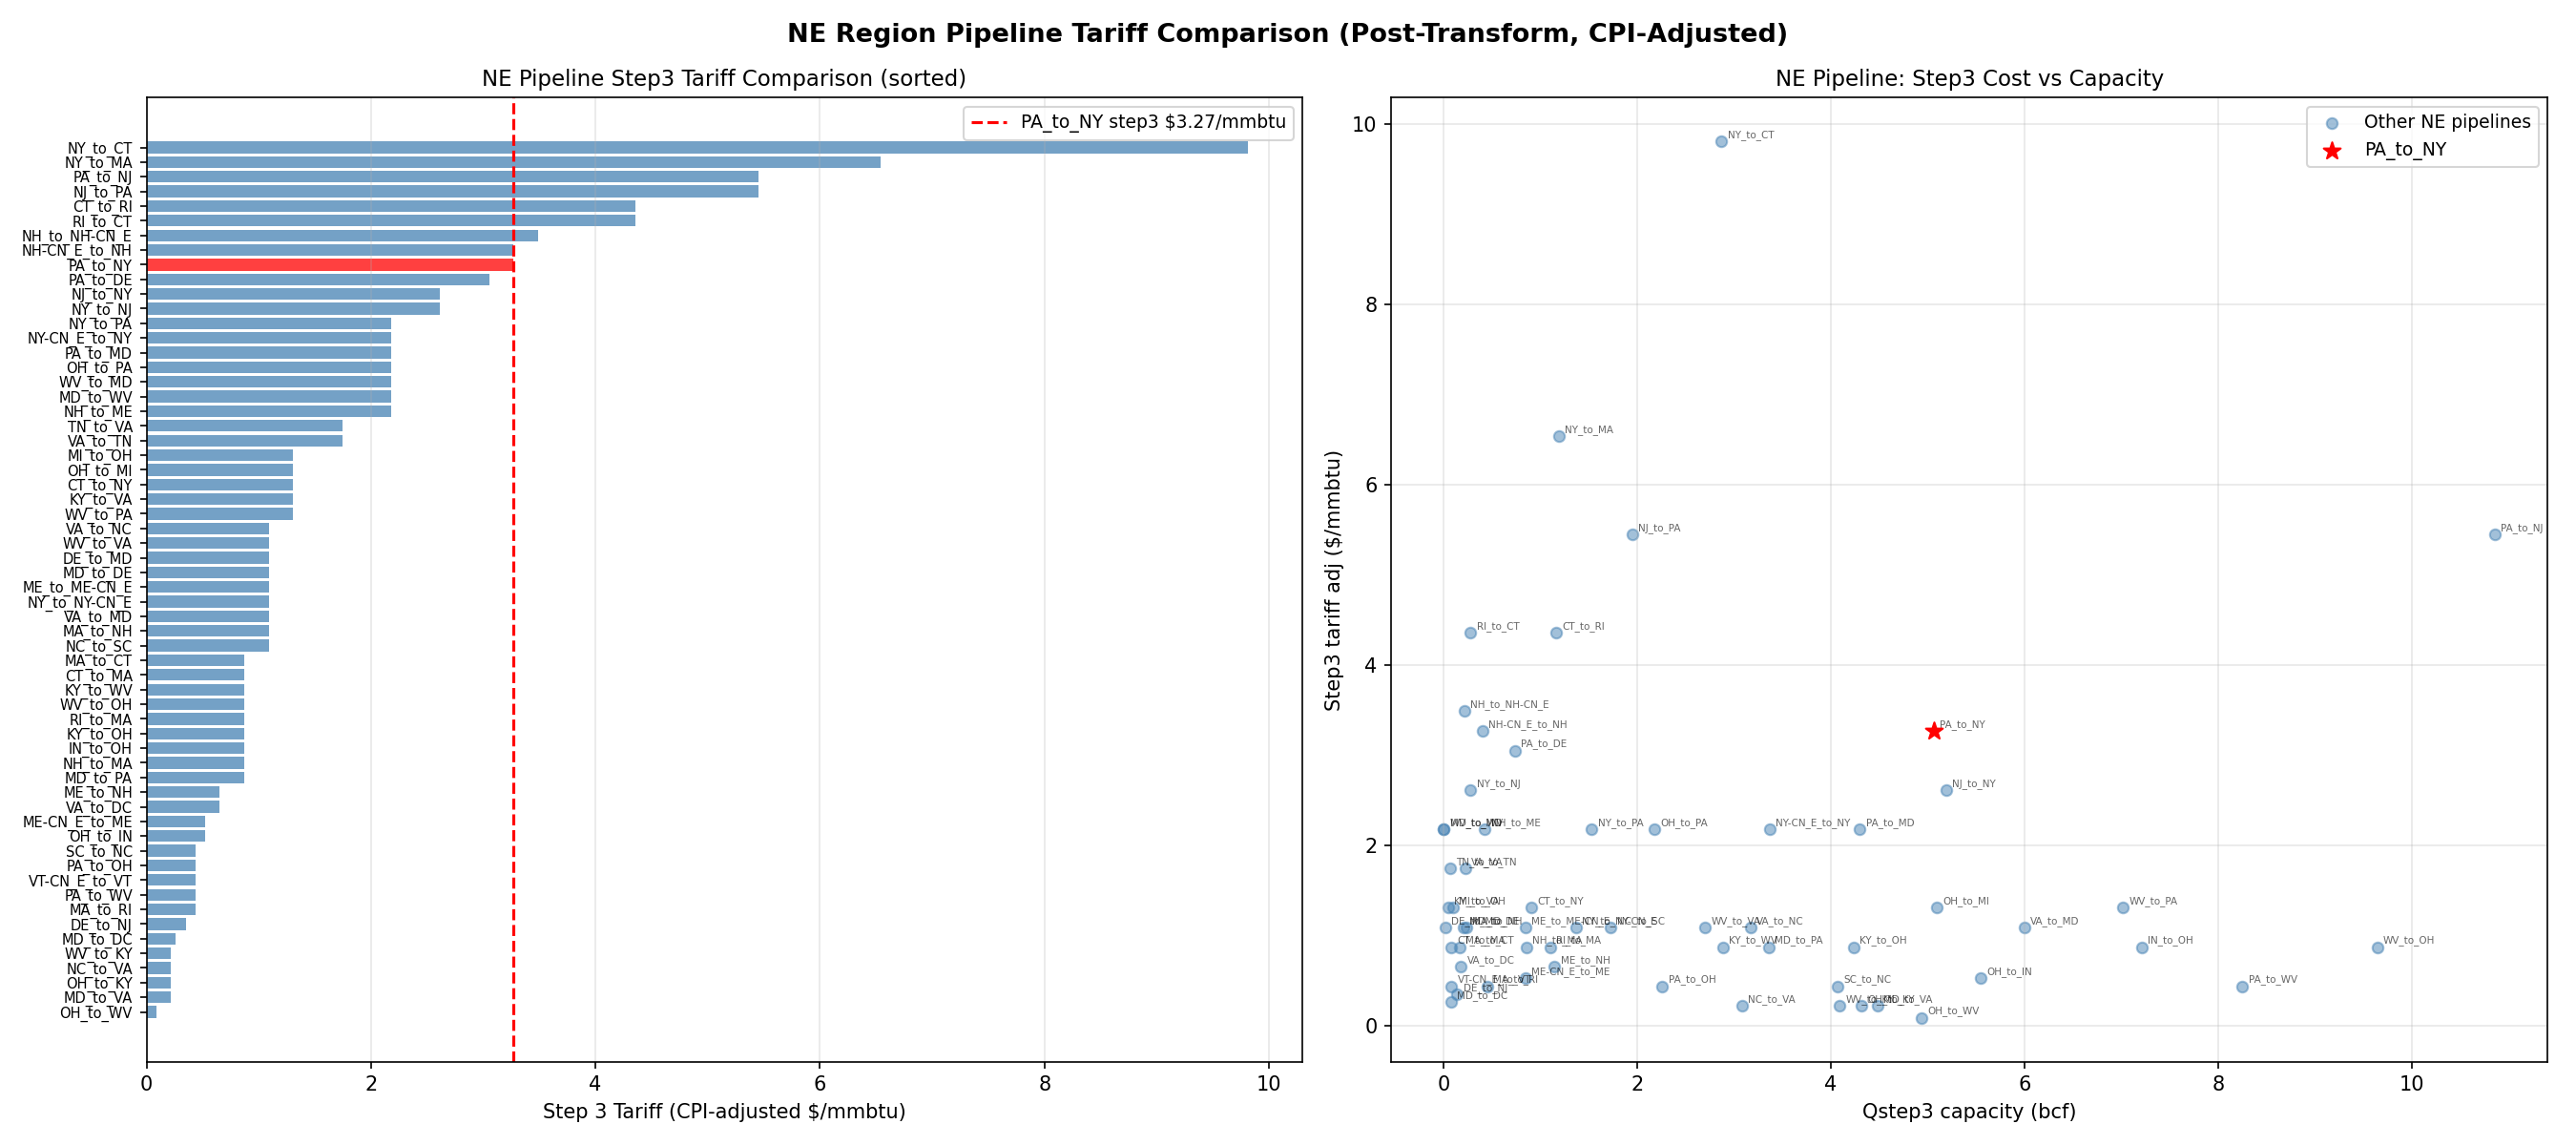
\includegraphics[width=0.88\linewidth]{pipe_04_ne_tariff_comparison.png}
  \end{figure}
  \vspace{-0.5em}
  {\small \textbf{Left}: step~3 CPI-adjusted tariff for all 60 NE-region pipelines. PA$\to$NY (red) is in the \textbf{top~12\%}. \textbf{Right}: scatter of step~3 cost vs.\ step~3 capacity --- PA$\to$NY is a high-capacity, high-cost outlier.}
\end{frame}

% ---- Slide 11: Inbound NY comparison ----
\begin{frame}{NY Inbound Pipelines: PA$\to$NY is the Jump Outlier}
  Among the 4 pipelines flowing \emph{into} NY:

  \vspace{0.3em}
  \begin{table}
    \centering
    \begin{tabular}{lcccr}
      \toprule
      \textbf{Pipeline} & \textbf{Step~2 adj} & \textbf{Step~3 adj} & \textbf{Step~3 width} & \textbf{Jump ratio} \\
      \midrule
      CT$\to$NY        & \$0.65 & \$1.31 & 0.091~bcf & 2.0$\times$ \\
      NY-CN\_E$\to$NY  & \$1.09 & \$2.18 & 1.011~bcf & 2.0$\times$ \\
      NJ$\to$NY        & \$1.31 & \$2.62 & 1.038~bcf & 2.0$\times$ \\
      \textbf{PA$\to$NY} & \textbf{\$0.22} & \alert{\textbf{\$3.27}} & \textbf{1.012~bcf} & \alert{\textbf{15.0$\times$}} \\
      \bottomrule
    \end{tabular}
  \end{table}

  \vspace{0.5em}
  \begin{itemize}
    \item PA$\to$NY has the \textbf{cheapest step~2} of any NY-inbound pipeline (\$0.22 vs.\ \$0.65--\$1.31)
    \item Its step~3 is the \textbf{most expensive} (\$3.27 vs.\ \$1.31--\$2.62) \\
    \item Every other NE pipeline has a 2$\times$ jump; PA$\to$NY jumps \textbf{15$\times$}
    \item This is economically plausible (firm vs.\ interruptible spread on Transco/Tennessee), \\
      but the magnitude may warrant rechecking against actual tariff filings
  \end{itemize}
\end{frame}

%% ============================================================
%% PART IV: SUMMARY
%% ============================================================

\section{Summary}

% ---- Slide 12: Verdict ----
\begin{frame}{Verdict and Implications}
  \begin{columns}[T]
    \column{0.5\textwidth}
      \textbf{\textcolor{okgreen}{What is NOT the issue}}
      \begin{itemize}
        \item[$\checkmark$] Code bug in \texttt{MaxPipe} constraint
        \item[$\checkmark$] Data-setup error in tariff transform
        \item[$\checkmark$] Incorrect values written to \texttt{.dat} file
        \item[$\checkmark$] Step~3 capacity never used \\
          {\small (used on 37 Part~2 days, 4 Part~3 days)}
      \end{itemize}

    \column{0.5\textwidth}
      \textbf{\textcolor{noteblue}{What is happening}}
      \begin{itemize}
        \item Most days: NY--PA spread $<$ \$3.27 \\
          $\Rightarrow$ step~3 not economical \\
          $\Rightarrow$ flow stops at 4.048~bcf
        \item High-demand days: spread $>$ \$3.27 \\
          $\Rightarrow$ optimizer correctly buys step~3 \\
          $\Rightarrow$ flow rises toward 5.060~bcf
        \item \textbf{Structural/economic result, \\
          not a model defect}
      \end{itemize}
  \end{columns}

  \vspace{0.8em}
  \begin{block}{Open calibration question}
    PA$\to$NY's 15$\times$ tariff jump (step~2: \$0.22 $\to$ step~3: \$3.27) is a notable outlier among NE pipelines. If this inflates congestion on this corridor, it may under-represent real PA$\to$NY flows during mild days. \textbf{Recommended}: cross-check against FERC tariff filings for Transco Zone~6 / Tennessee 300~Line.
  \end{block}
\end{frame}

% ---- Slide 13: Summary table ----
\begin{frame}{Diagnostic Checklist}
  \begin{table}
    \centering
    \begin{tabular}{llc}
      \toprule
      \textbf{Check} & \textbf{Method} & \textbf{Result} \\
      \midrule
      Step~3 capacity ever used? & Script~01 flow distribution & \textcolor{okgreen}{\textbf{Yes, 37 Part~2 days}} \\
      Conflict days (gap $>$ cost, flow capped)? & Script~02 dual gap test & \textcolor{okgreen}{\textbf{0 days}} \\
      Tariff values correct in \texttt{.dat}? & Script~03 file parse & \textcolor{okgreen}{\textbf{PASS}} \\
      PA$\to$NY step~3 jump normal? & Script~04 NE comparison & \textcolor{alertred}{\textbf{Outlier (15$\times$)}} \\
      \midrule
      \textbf{Bug verdict} & & \textcolor{okgreen}{\textbf{No bug}} \\
      \textbf{Calibration flag} & & \textcolor{alertred}{\textbf{15$\times$ jump to review}} \\
      \bottomrule
    \end{tabular}
  \end{table}
\end{frame}

\end{document}
